% lecture12.tex — Mod 2 Intersection Theory

\section{Mod 2 Intersection Theory}

Consider two closed submanifolds $M_1, M_2 \subset N$ of complementary dimension (i.e.\ $\dim M_1 + \dim M_2 = \dim N$), where at least one of $M_1$ or $M_2$ is compact.

When they intersect transversely, $M_1 \cap M_2$ must be a compact $0$-manifold (i.e.\ a finite set of points), so we can count the ``intersection number'' $\#(M_1 \cap M_2)$.

Even if their intersection is not transverse, we know we can homotope them to make it transverse.

\begin{center}
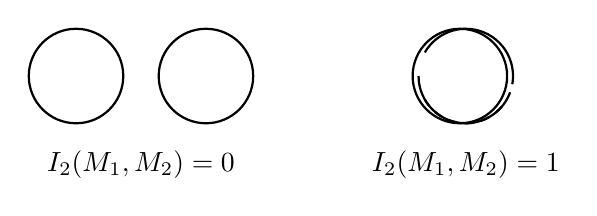
\begin{tikzpicture}[scale=0.75]
    % Unlinked circles
    \draw[thick] (0,0) circle (0.8);
    \draw[thick] (2.2,0) circle (0.8);
    \node at (1.1,-1.5) {$I_2(M_1, M_2) = 0$};
    % Linked circles
    \begin{scope}[xshift=6.5cm]
        \draw[thick] (0,0) circle (0.8);
        \draw[thick] (0.9,0) arc(0:150:0.8);
        \draw[thick,dashed] (0.9,0) arc(0:-150:0.8);
        \draw[thick] (-0.7,0) arc(180:330:0.8);
        \node at (0.1,-1.5) {$I_2(M_1, M_2) = 1$};
    \end{scope}
\end{tikzpicture}
\end{center}

Depending on the choice of homotopy, the number of intersections might change, but we'll show that the \emph{mod 2 intersection number} is well-defined.

\begin{definition}{Mod 2 Intersection Number}{mod2-intersection}
    Suppose $M_1$ is a compact manifold, $f \colon M_1 \to N$ is a smooth map, $M_2 \subset N$ is a closed submanifold with $\dim M_1 + \dim M_2 = \dim N$. Choose any map $g$ homotopic to $f$ and transversal to $M_2$. Define the \emph{mod 2 intersection number} of $f$ with $M_2$, $I_2(f, M_2)$, to be
    \[
        \# g^{-1}(M_2) \mod 2 \quad \in \Z/2\Z.
    \]
\end{definition}

\begin{theorem}{Mod 2 Intersection Number is Well-Defined}{mod2-well-defined}
    If $g_0, g_1 \colon M_1 \to N$ are homotopic and both transversal to $M_2 \subset N$, then $\# g_0^{-1}(M_2) = \# g_1^{-1}(M_2) \mod 2$.

    In particular, the mod 2 intersection number is well-defined and invariant under homotopy.
\end{theorem}

\begin{proof}
    Let $G \colon M_1 \times I \to N$ be a homotopy of $g_0$ and $g_1$. By the relative transversality homotopy theorem, we may assume $G \pitchfork M_2$. Then $G^{-1}(M_2)$ is a 1-dimensional submanifold of $M_1 \times I$ with boundary
    \[
        \partial G^{-1}(M_2) = G^{-1}(M_2) \cap \partial(M_1 \times I) = g_0^{-1}(M_2) \times \{0\} \cup g_1^{-1}(M_2) \times \{1\}.
    \]
    \begin{center}
    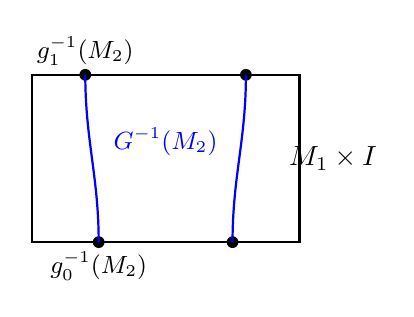
\begin{tikzpicture}[scale=0.85]
        % M_1 x I rectangle
        \draw[thick] (0,0) rectangle (4,2.5);
        \node at (4.5,1.25) {$M_1 \times I$};
        % Bottom: g_0^{-1}(M_2)
        \fill (1,0) circle (2.5pt) node[below] {\small $g_0^{-1}(M_2)$};
        \fill (3,0) circle (2.5pt);
        % Top: g_1^{-1}(M_2)
        \fill (0.8,2.5) circle (2.5pt) node[above] {\small $g_1^{-1}(M_2)$};
        \fill (3.2,2.5) circle (2.5pt);
        % Cobordism curves
        \draw[thick,blue] (1,0) to[out=90,in=270] (0.8,2.5);
        \draw[thick,blue] (3,0) to[out=90,in=270] (3.2,2.5);
        \node[blue] at (2,1.5) {\small $G^{-1}(M_2)$};
    \end{tikzpicture}
    \end{center}
    Since the boundary of any compact 1-manifold has an even number of points, $\# g_0^{-1}(M_2) + \# g_1^{-1}(M_2)$ is even.
\end{proof}

\begin{example}{Mod 2 Intersection Numbers}{mod2-examples}
    \begin{enumerate}
        \item Let $D \subset \R^3$ be a disk and $S^1 \subset \R^3$ a circle, with $\partial D$ unlinked from $S^1$. Then $I_2(D, S^1) = 0$, since $D$ may be chosen disjoint from $S^1$. (Dim check: $\dim D + \dim S^1 = 2 + 1 = 3 = \dim \R^3$.)
        \item Let $D \subset \R^3$ be a disk and $S^1 \subset \R^3$ a circle, with $\partial D$ linked with $S^1$. Then $I_2(D, S^1) = 1$, since every disk bounded by $\partial D$ must be punctured by $S^1$ an odd number of times.
        \item The core circle $M$ of a M\"obius band $N$: the mod 2 self-intersection number $I_2(M, M) = 1$.
    \end{enumerate}
\end{example}

% Examples are illustrated by the linked/unlinked diagrams above and the Mobius band diagram below

\subsection{Boundary Theorem}

\begin{theorem}{Boundary Theorem}{boundary-thm}
    Suppose that $M_1$ is the boundary of some compact manifold $W$ and $f \colon M_1 \to N$ is a smooth map. If $f$ can be extended to all of $W$, then $I_2(f, M_2) = 0$ for any closed submanifold $M_2 \subset N$ of complementary dimension.
\end{theorem}

\begin{proof}
    Let $F \colon W \to N$ extend $f$, which we may assume to be transversal to $M_2$, by the transversality homotopy theorem. Then $F^{-1}(M_2)$ is a compact 1-manifold with boundary $\partial F^{-1}(M_2) = f^{-1}(M_2)$, so $\# f^{-1}(M_2)$ must be even.
    \begin{center}
    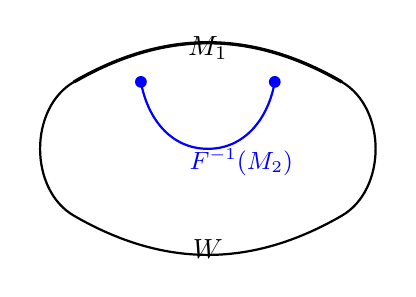
\begin{tikzpicture}[scale=0.85]
        % W (blob)
        \draw[thick] (0,0) to[out=30,in=150] (4,0) to[out=-30,in=30] (4,-2) to[out=210,in=330] (0,-2) to[out=150,in=210] cycle;
        \node at (2,-2.5) {$W$};
        % M_1 = boundary (top part)
        \draw[very thick] (0,0) to[out=30,in=150] (4,0);
        \node at (2,0.5) {$M_1$};
        % F^{-1}(M_2) curves with boundary on M_1
        \draw[thick,blue] (1,0) to[out=-80,in=180] (2,-1) to[out=0,in=260] (3,0);
        \fill[blue] (1,0) circle (2.5pt);
        \fill[blue] (3,0) circle (2.5pt);
        \node[blue] at (2.5,-1.2) {\small $F^{-1}(M_2)$};
    \end{tikzpicture}
    \end{center}
\end{proof}

\subsection{Mod 2 Degree}

\begin{definition}{Mod 2 Degree}{mod2-degree}
    If $f \colon M \to N$ is a smooth map of a compact manifold $M$ into a connected manifold $N$ of the same dimension, define the \emph{mod 2 degree} of $f$,
    \[
        \deg_{\Z/2}(f), \text{ to be } I_2(f, \{y\}), \text{ for any point } y \in N.
    \]
\end{definition}

\begin{theorem}{Mod 2 Degree is Well-Defined}{mod2-degree-well-defined}
    Mod 2 degree is well-defined.
\end{theorem}

\begin{proof}
    For any $y \in N$, we can homotope $f$ to make it transversal to $\{y\}$. From Lecture 4, we know $y \mapsto I_2(f, \{y\})$ is locally constant. Since $N$ is connected, it must be globally constant.
\end{proof}

Since $\deg_{\Z/2}$ is defined as an intersection number, we immediately obtain:

\begin{theorem}{}{mod2-degree-homotopy}
    The mod 2 degree is invariant under homotopy.
\end{theorem}

\begin{theorem}{}{mod2-degree-boundary}
    If $M = \partial W$ and $f \colon M \to N$ extends to all of $W$, then $\deg_{\Z/2}(f) = 0$.
\end{theorem}

\begin{example}{Mod 2 Degree Examples}{mod2-degree-examples}
    A constant map $c \colon M \to M$, $x \mapsto c$, has $\deg_{\Z/2}(c) = 0$.

    The identity map $\id \colon M \to M$, $x \mapsto x$, has $\deg_{\Z/2}(\id) = 1$.

    In particular, the identity map of a compact manifold (without boundary) is NOT homotopic to a constant map.

    (In case $M = \partial W$, this implies that $\id \colon M \to M$ cannot be extended to all of $W$, a result we saw in Lecture 10.)
\end{example}
